\documentclass[11.5pt]{sig-alternate}
\usepackage[defaultlines=3,all]{nowidow}
\usepackage{hyperref}
\usepackage{tabularx}
\usepackage{graphicx}
\usepackage{blindtext}
\usepackage[utf8]{inputenc}
\usepackage[english]{babel}
\usepackage{lastpage}
\usepackage{comment}
\usepackage{dirtytalk}
\usepackage{xcolor}
\usepackage{hanging}
\usepackage{wrapfig}
\usepackage[backend=biber, style=apa]{biblatex}
\addbibresource{notation.bib}
\usepackage{authblk}
\usepackage{caption}
\usepackage{graphicx,subfigure}
\usepackage{authblk}
\usepackage{enumitem}
\usepackage[utf8]{inputenc}
\usepackage{cuted}
\usepackage{fancyhdr}
\pagestyle{fancy}
\usepackage{lipsum}
\renewcommand{\headrulewidth}{0pt}
\renewcommand{\footrulewidth}{0pt}
\setlength\headheight{80.0pt}
\addtolength{\textheight}{-80.0pt}
\chead{%
  \ifcase\value{page}
  % empty test for page = 0
  \or 
\includegraphics[width=\textwidth]{headerImage.png}% page = 1
  \or 
\includegraphics[width=\textwidth]{headerImage.png}% page = 2
  \or 
\includegraphics[width=\textwidth]{headerImage.png}% page = 3
  \or 
\includegraphics[width=\textwidth]{headerImage.png}% page = 4
  \or 
\includegraphics[width=\textwidth]{headerImage.png}% page = 5
  \else
  
\includegraphics[width=\textwidth]{headerImage.png}
  \fi
}

%\chead{\includegraphics[width=\textwidth]{JSESD Island Conference Article banner-02.jpg}}
\fancyfoot[LE,LO]{An Introductory Course in Electrical Circuits and Coding for Deaf and DeafBlind Middle School Students\\           
DOI: 10.14448/jsesd.15.0008}
\fancyfoot[CE,CO]{{ }}
\fancyfoot[RE,RO]{\thepage}
\pagenumbering{arabic}
\hypersetup{
    colorlinks=true,
    urlcolor=blue
}
 
\let\oldabstract\abstract
\let\oldendabstract\endabstract
\makeatletter
\renewenvironment{abstract}
{\renewenvironment{quotation}%
               {\list{}{\addtolength{\leftmargin}{1em} % change this value to add or remove length to the the default
                        \listparindent 1.5em%
                        \itemindent    \listparindent%
                        \rightmargin   \leftmargin%
                        \parsep        \z@ \@plus\p@}%
                \item\relax}%
               {\endlist}%
\oldabstract}
{\oldendabstract}
\makeatother

% Left align captions
\captionsetup{justification   = raggedright,
              singlelinecheck = false}


\begin{document}

\title{An Introductory Course in Electrical Circuits and Coding for Deaf and DeafBlind Middle School Students}

\author[0]{\large \color{blue} Becca Leininger}
\author[1]{\large \color{blue}Christina Yang}
\author[1]{\large \color{blue}Makayla Quinn}
\author[1]{\large \color{blue}Jeffrey Jalkio}
\author[1]{\large \color{blue}Rahaf Bahajry}
\author[1]{\large \color{blue}Mellissa Ingabire}
\author[1]{\large \color{blue}AnnMarie Thomas}
\affil[1]{University of St. Thomas- Minnesota}
\toappear{}

\maketitle
\begin{@twocolumnfalse} 
\begin{abstract}
\item 
 \textit{The Playful Learning Lab collaborated with Metro Deaf School (MDS) to design and deliver an Intro to Electronics and Computer Programming course to Deaf and DeafBlind middle school students. Four sets of 6–8 students went through an approximately 20-day course that met four days a week for 40 minutes per day. The content of the class focused on electrical circuits and computer programming. Lessons covered topics such as conductivity, closed/open circuits, series/parallel circuits, and coding. Students were introduced to the Scratch computer programming language and Makey kits. The development and delivery of the course was a collaborative effort between Metro Deaf School staff and the undergraduate student researchers in the Playful Learning Lab. The class was a project based mix of lectures, projects, and
hands-on assignments. In this presentation we will share the lessons learned by designing, and delivering, this course.}
     \\
     \\
     Keywords: Engineering, Deaf, Circuits
\end{abstract}
\end{@twocolumnfalse}

%% ABSTRACT


%% AUTHOR INFORMATION


\textbf{*Corresponding Author,  Becca Leininger}\\
\href{mailto: lein6470@stthomas.edu}{(lein6470@stthomas.edu)} \\
\textit{Submitted Thu Apr 6 2023 }\\
\textit{Accepted Mon Aug 21 2023} \\
\textit{Published online } \\
\textit{DOI: 10.14448/jsesd.15.0008} \\
\pagebreak
\pagebreak

\vspace{5mm}
\section*{\vspace{140mm}}
\begin{large}
    \section*{An Introductory Course in Electrical Circuits and Coding for Deaf and DeafBlind Middle Sch-ool Students}
Metro Deaf School (MDS) in St. Paul, Minnesota is the first Deaf charter school in the United States, opening in 1993. The school serves students in the Twin Cities and Western Wisconsin from ages 2 to 21 who are primarily Deaf, DeafBlind and Hard of Hearing students, often being visual and/or tactile learners. All students who attend MDS have Individualized Education Plans (IEPs) and fall under the \textit{special education} category, defined by the Minnesota Department of Education as students who “have a disability and need specialized instruction” (Minnesota Department of Education, n.d.). At MDS, students are instructed in American Sign Language (ASL) and English is primarily taught through print.

The Playful Learning Lab (PLL) is an undergraduate student research lab at the University of Saint Thomas in St. Paul, Minnesota. Members of the PLL come from a variety of majors such as education, engineering, and psychology. Student researchers collaborate to promote learning through play on projects such as Circus Science (Roche et al., 2020), The PLAYground (Monson et al., 2020), and OK GO Sandbox (Schumacher et al., 2020). The PLL frequently collaborates with community partners such as The Minnesota Children’s Museum, Tw-in Cities Trapeze, and Metro Deaf School.

The PLL has been working with MDS for over 8 years, starting with after-school STEAM workshops for students to engage in engineering \\ projects outside their normal curriculum (Kas-per et al., 2016). In 2020, the PLL worked with MDS to host an online PLAYground camp for students in the wake of the COVID-19 pandemic (Monson et al., 2021). Ongoing research through this collaboration include teacher workshops exploring the Scratch programming language through videos presented in ASL and \\ LEGO Spike Prime with their students.

\section*{ Course Development}
\textbf{\textit{ Curriculum Goals}}

In this collaboration, our goal was to design and assist in teaching a 16-21 day Intro to Electronics and Computer Programming class to Deaf and DeafBlind middle school students in four rotations of 7 students each (N=28). These classes provided hands-on materials to encourage learning through play, implemented inquiry-based learning, and gave students the time to explore and undergo their own learning process. The first portion of the class focused on engineering and circuits. This was taught using Squishy Circuits (Peppler et al., 2018; Johnson et al., 2010) and Paper Circuits from Brown Dog Gadgets. The topics covered series and parallel circuits, open and closed circuits, switc-hes, and basic vocabulary including batteries, LEDs, conductors, and insulators. Topics also included safety relating to circuitry.

The second portion of the class was centered on the Scratch programming language (Resnick et al., 2009). The first lesson introduced students to the coding language before allowing them to explore the online Scratch community and to create their own coding projects. Video tutorials were used to introduce projects to students and serve as a guide if they needed help. The coding lessons included animating your name, creating a chase game, and a final project of creating their own game using a Makey Makey, an invention kit designed to allow conductive objects to serve as computer control inputs, as a game controller.
\newpage
\textbf{\textit{Planning the Course }}

During the month of January 2022, student researchers and faculty partners began to develop content for the Intro to Electronics and Computer Programming class. The development team, consisting of mechanical and electrical engineering, education, and entrepreneurship perspectives, brainstormed key electrical engineering and computer programming concepts to cover in the course. It was important for our team to include student researchers with varying levels of content knowledge to refine and simplify the curriculum in a way that was appropriate for middle school students. One method of this refining process involved associating key topics with everyday objects and images, connecting potentially abstract content with relatable, concrete concepts. For example, when introducing the idea of electrical current we compared it to water flowing through pipes. This focus on key topics, and key vocabulary words, was supported heavily by the classroom teacher. Because the classroom had open wall space, we created large-print vocabulary posters to put on the wall of the classroom for the students to reference.The teaching team, which included the student researchers, faculty partners, and the classroom teacher, focused the curriculum around pre-existing interactive activities to provide students a way to associate their experiences with the electrical engineering and computer science content.

The coding activities utilized in the second half of the course were centered around the lessons and activities on the Scratch website and the Creative Coding Curriculum (Brennan et al., 2011). We selected activities and ideas that would inspire students to have the flexibility to creatively express themselves and develop their problem-solving skills. The diverse backgrounds and disciplines of the teaching team helped to break down the concepts to simple, concrete ideas that could be emphasized in the curriculum as it was being developed. During the planning phase, it was crucial for us to include hands-on activities that would reinforce the content of the curriculum to provide the students the opportunity to learn through play. To evaluate the success of this course, we took two approaches: responding to the needs of the students in real time (further explored in the discussion section) and evaluating interest and confidence in the subjects covered as well as concept knowledge before and after the course.

\section*{ Method}

On the first day of each of the four rotating sessions of the course, each session with 7 students each (N=28), students were given a presentation on the process of the course and the researcher’s goal of evaluating student interest and confidence in subject skills through the \\ course. They were also given information on assent and consent forms, approved by the Institutional Review Board at the University of St. Thomas, were sent to parents. Students who assented were given a pre-test consisting of fourteen 5-point Likert scale questions on subject interest and confidence, and eight fill-in-the-blank concept questions pertaining to electrical engineering and computer programming with a provided word bank (See Appendix A).

The exact same post-test was given on the final days of the class while students were finishing their final projects. The students were informed that these tests would not impact their grade and were for research purposes only. The pre- and post-tests were then analyzed to determine if students’ attitudes and interest towards engineering and computer science changed throughout the course as well as students' knowledge of the content. The subject interest questions were recoded into disagree (Strongly Disagree and Disagree), not sure (Neither Agree or Disagree), and agree (Strongly Agree and Agree).

\section*{ Quantitative Results}

Due to absences resulting in missing pre- and post-test data, subject interest questions use data from 18 students and the concept questions use data from 13 students. To test the significance of the pre-test scores compared to the post-test scores, we used a paired-samples t-test. We also adopted a significance level of 0.1 due to low statistical power caused by the small number of participants for both the interest questions (N=18) and the concept questions (N=13). There was not a significant change between pre-test (M=45.75, SD=8.17) and post-test (M=45.93, SD=8.27) scores for subject interest and confidence, t(12) = 0.186, p > 0.1, two-sided. To determine changes in interest question responses, we looked at the frequency for each category. Students indicated agreement more often in the post-test (42.6\%) than in the pre-test (35.2\%) for engineering interest and ability questions (See Figure 1).
\section*{Figure 1}
\textit{Engineering Question Agreement Frequency}
\begin{figure}[h!]
\centering
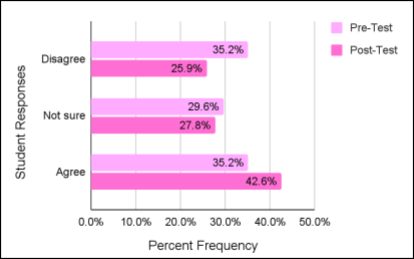
\includegraphics[width=8cm]{figure 1.png}
\end{figure}

Students indicated agreement less often in the post-test (58.3\%) than in the pre-test (63.9\%) for math interest and ability questions \\(See Figure 2). 
\section*{Figure 2}
\textit{Computer Science Agreement Frequency}
\\
\begin{figure}[h!]
\centering
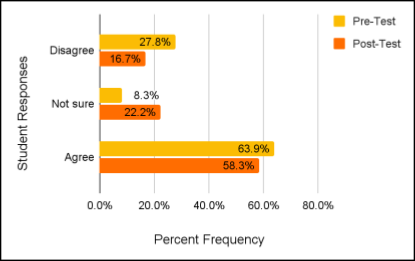
\includegraphics[width=8cm]{figure 2.png}
\end{figure}

It is important to note that although agreement frequency decreased in the math post-test, there were more of those who were not sure (22.2\%) compared to those that disagreed (16.7\%).
Students indicated agreement less often in the post-test (22.2\%) than the pre-test (27.8\%) for the computer science interest and ability questions (See Figure 3).

\section*{Figure 3}
\textit{Math Question Agreement Frequency}

\begin{figure}[h!]
\centering
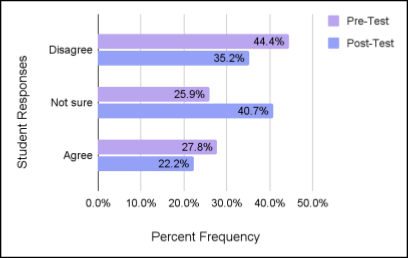
\includegraphics[width=7.5cm]{figure 3.png}
\end{figure}

Similar to the math results, there were more students that were not sure (40.7\%) in the post-test than students who disagreed (35.2\%). Students indicated agreement more often in the post-test (57.4\%) than in the pre-test (53.7\%) for problem-solving interest and ability questions (See Figure 4).

\section*{Figure 4}
\textit{Problem-Solving Agreement Frequency}
\\
\begin{figure}[h!]
\centering
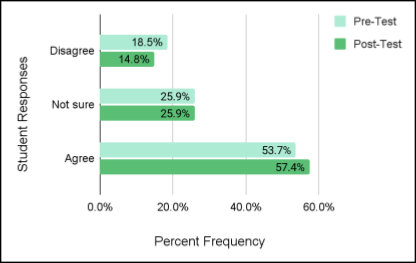
\includegraphics[width=8cm]{figure 4.png}

\end{figure}

There was a significant increase between the pre-test scores (M=1.08, SD=1.38) and the post-test scores (M=4.46, SD=2.11) for the concept questions, t(12)=6.034, p < 0.1, one-sided (See Figure 5).

\section*{Figure 5}
\textit{Total Mean Score of Concept Questions}
\begin{figure}[h!]
\centering
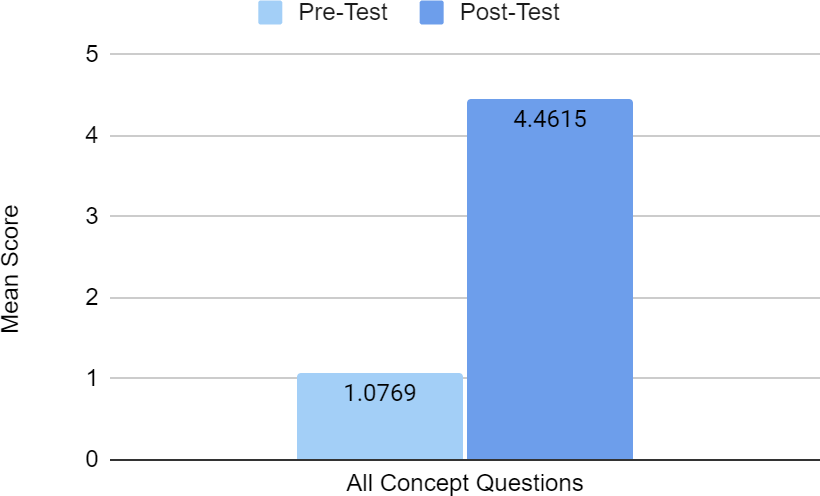
\includegraphics[width=8cm]{figure 5.png}
\end{figure}

\textit{Note: Each question was scored as either 0 = incorrect or 1 = correct. There were 8 questions total. The minimum score possible was 0 and the maximum score was 8.}

Students not only had more correct answers in the post-test, but wrote something in the answer space which was frequently left blank in the pre-test. Each concept question had more correct answers after students took the course (See Figure 6).
\\
\\
\section*{Figure 6}
\textit{Mean Score of Individual Concept Questions}
\begin{figure}[h!]
\centering
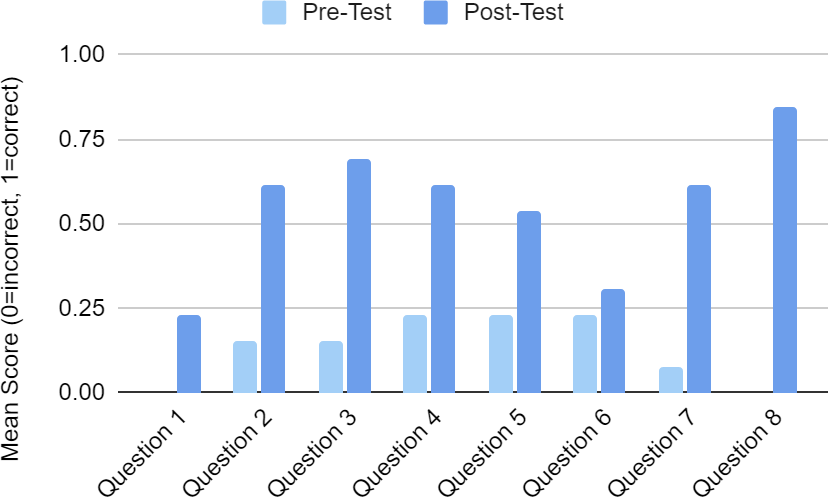
\includegraphics[width=8cm]{figure 6.png}

\end{figure}

\section*{ Discussion}
\subsection*{Results Summary}
It can be hypothesized that students answered more questions correctly when the content contained recurring visual images, as in the lessons on circuit types and components.
\subsection*{Accessibility Learnings}

As discussed in the Curriculum Goals section, it was important for us to notice student responses to the design of the course and address their learning needs by adapting our teaching methods. Because the course was created by hearing individuals, this step was important to make the course accessible for all students. One example was our slideshow used to teach lessons which needed to be viewer friendly, particularly for DeafBlind students. Our original design utilized an engineering themed slideshow, which was heavy on background images and colors in the templates. This, however, proved to affect the lack of clarity of the slides due to busy design graphics. With guidance from the classroom teacher and a faculty partner, the slides were redesigned - including changing the background and text colors to that more suitable for DeafBlind students, larger font sizes, and clear visuals for important concepts.

As the school year progressed and the teaching team was able to teach more students, more adaptations were required to ensure all students could use the materials. In the fourth group of students, for example, one student had difficulty with fine motor skills and was not able to manipulate the supplies to complete the paper circuit activities. 
\renewcommand{\thefigure}{7}
\begin{figure}[h!]
\centering
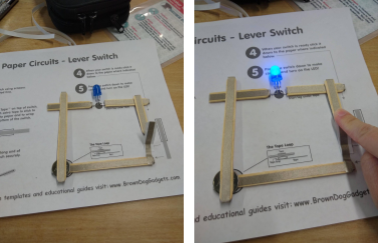
\includegraphics[width=8.5cm]{figure 7.png}
\caption{ Demonstration of an accommodation created for a student to be able to participate in the Paper Circuit activities. Student researchers wrapped the conductive tape around popsicle sticks that the student was able to manipulate with the help of their paraprofessional.}
\end{figure}
\\ In searching for a solution for this student, our researchers came up with putting the conductive tape on popsicle sticks the student could move around and manipulate much easier (See Figure 7). With the help of the student’s paraprofessional, they were able to complete the activities and explore the circuits using the popsicle sticks to connect the battery to the LEDs.

Another unexpected change was moving the \\course online, as the school went to distance learning due to an increase of COVID cases during the first week of the 4th rotation. Two days prior to this change, the teaching team, as well as school teachers and paraprofessionals, packaged and distributed a week’s worth of materials for the students to ensure all students had the tactile tools used to instruct the lessons. This distribution was important as we recognized the possibility of students not having access to the same materials at home as used in the classroom. Additionally, the teaching team had their own set of materials to help the teaching team demonstrate the concepts and activities over Zoom. The flow of the class changed while online to accommodate for technical difficulties and the time needed for students to work at their own pace. We did experience technical difficulties with administering the pre-test for rotation 4 through Kami, which allowed students to annotate a digital version of the test accessibly.

For this online format, the teaching team spent some time on the first day going through our bag of materials as a class, which engaged the students and sparked excitement and curiosity for the activities we would be working on. While sharing the slides on the screen, a team member angled their camera to demonstrate the concepts taught using Squishy Circuits dou-gh and LEDs. With the adjustment in the duration of the class, we were intentional about giving students additional time to participate in the activities at home. When we saw that students were stuck while building, the classroom teacher pointed out different approaches students took and emphasized the idea that there was no “right way” to approach the activities in class. This creative thinking was embraced by the students. One student, for example, did not have insulating dough in their materials, so they came up with the innovative idea of using a plastic lid as their insulator in our Squishy Circuits activity.
\section*{ Limitations}
\textbf{\textit{The Course}}

To begin, we wanted to note that these Deaf and Hard of Hearing students were assessed by a survey and course created by hearing individuals. While we intended to create a course that was optimal for these students, we recognize that there may have been shortcomings in the resources and content.The ASL signs needed to teach the content were not widely known in the community we worked with. This allowed for us to collaborate with the classroom teacher to create ASL signs to describe series and parallel circuits, some of the most common vocabulary used in the class. When the students were taking the post-test, many of them were able to explain the concepts correctly in ASL, but could not remember the English word to write on the test. Similarly, we observed that students were better able to understand concepts when multiple visuals were present and repeated throughout the content. Especially in the lessons on circuit types and components, more students were able to correctly identify the circuit images in the post test out of the other concept questions. We correlate this finding to the increased and repeated use of visuals in the lessons on circuits and the importance of visuals in successful learning of Deaf and Hard of Hearing students.
\newpage
\textbf{\textit{The Study}}

Due to the COVID-19 pandemic, the class had unpredictable student absences leading to incomplete data collection for all 28 students. This reduced number of participants could impact the validity of the results as well as the differences in instruction received in the first week of rotations 1-3 (in-person) vs rotation 4 (online). The questions for the subject interest section of the pre- and post-tests were created by the authors, and there may be a limitation in inference validity. The present study represents a first attempt to represent the success and need for this course in Deaf and DeafBlind education. We feel that further research examining accessible teaching methods and data collection may open possibilities for further work and research.
\newpage
\section*{ Conclusion}

The development and implementation of the Introduction to Electronics and Computer Programming course was a stepping stone to accessible STEM and computer science courses for Deaf and Hard of Hearing students. We gained valuable insights on how students feel about the topics they are taught and the influence of our instruction methods on the students and their learning. Through our research, we reinforced the idea that Deaf and Hard of Hearing students benefit from the inclusion of multiple visuals when learning content, especially new content in complex content areas. Students also benefit when they have the full signing vocabulary of the content area, something that is sometimes lacking in STEM content (Bigham et al., 2008). Deaf and Hard of Hearing students require attentive and accessible materials to assist them in learning and understanding content, and we hope to continue to meet these needs through empowering children with playful education.
\newpage
\section*{ Acknowledgements}

The authors would like to thank the many individuals and groups that assisted with this work and paper. This includes Dr. Douglas Orzolek for consulting on pedagogy, Dr. Elise Amel for her assistance in data analysis, Maria Johnson for creating the slides used in this course, and all members of the Playful Learning Lab who assisted with materials preparation and review. We are grateful to Metro Deaf School educator Sandy Culpepper for working closely with us on this course, and Dr. Susan Outlaw for her partnership on this collaboration. Brown Dog Gadgets and Squishy Circuits donated materials that were used in this program. We also thank the Google Computer Science Education Research program for funding that made this work possible.

\end{large}
\include{} 
\section*{ References}\par 

\leftskip 0.25in
\parindent -0.25in 

Bigham, J. P., Otero, D. S., DeWitt, J. N., Cavender, A. C., \& Ladner, R. E. (2008). ASL-STEM forum: A bottom-up approach to enabling American Sign Language to grow in STEM fields. \textit{Second International AAAI Conference on Weblogs and Social Media}, 2(1)176-177. \\https://doi.org/10.1609/icwsm.v2i1.18638

Brennan, K., Balch, C., \& Chung, M. (2014). \textit{ Creative computing: A design-based introduction to computational thinking}. Harvard Graduate School of Education. \\https://creativecomputing.gse.harvard.edu/guide/

Johnson, S., \& Thomas, AM. (2010). Squishy Circuits: A tangible medium for electronics education. ACM Conference on Computer Human Interactions, Atlanta, GA.

Kasper, B., Haugh, A., Kasper, N., Gunderson, B., Thomas, AM., \& Besser, D. (2016). Design, implementation, and assessment of an after-school engineering program for deaf students. ASEE Annual Conference, New Orleans, LA.

Monson, E., Schumacher, K., \& Thomas, A. M. (2021). The playground: An online summer camp for deaf and hard of hearing children. \textit{Journal of Science Education for Students with Disabilities}, 24(1), 1–6. \\https://doi.org/10.14448/jsesd.13.0008

Minnesota Department of Education (n.d.). \textit{Special education}.https://education.mn.gov/MDE/fam/sped/

Peppler, K., Wohlwend, K., Thompson, N., Tan, V., \& Thomas, AM. (2018). Squishing circuits: Circuitry learning with electronics and playdough in early childhood. Journal of Science Education and Technology, 28(2), pp. 118-132. https://doi.org/10.1007/s10956-018-9752-2

Resnick, M., Maloney, J., Monroy-Hernández, A., Rusk, N., Eastmond, E., Brennan, K., Millner, A., Rosenbaum, E., Silver, J., Silverman, B., \& Kafai, Y. (2009). Scratch: Programming for all. \textit{Communications of the ACM}, 52(11), 60-67. \\https://doi.org/10.1145/1592761.1592779

Roche, P., Goldbach, C. J., Putman, A., Jalkio, J. A., Kimball, K., \& Thomas, A. M. P. (2020). Circus science. \textit{Proceedings of the Fourteenth International Conference on Tangible, Embedded, and Embodied Interaction}. \\https://doi.org/10.1145/3374920.3374986

Schumacher, K., Roche, M., Verschoor, E., French, H., Eggersgluss, A., Harjamaki, M. K., Fagot, M., Jalkio, J., Thomas, A. M., Goldbach, C., Besser, D., \& Bensen, A. (2020). Using music videos to inspire engineering.\textit{ 2020 ASEE Virtual Annual Conference Content Access Proceedings}. https://doi.org/10.18260/1-2--35466

 
\begin{large}
\twocolumn
\section*{ Appendix A}
Subject Interest Questions

\subsection*{Engineering Questions}
\begin{enumerate}
  \item I could be an engineer.
  \item I like engineering.
  \item I am good at engineering.
\end{enumerate}

\subsection*{Computer Science Questions}
\begin{enumerate}
  \item I could be a computer programmer.
  \item I like computer programming.
  \item I am good at computer programming.
\end{enumerate}

\subsection*{Math Questions}
\begin{enumerate}
  \item I like math.
  \item I am good at math.
\end{enumerate}

\subsection*{Problem Solving  Questions} 
\textit{Note:} Underlined words were fill-in-the-blank with answers being present in a word bank. I like learning how things work.
\begin{enumerate}
    \item I am good at learning how things work.
    \item I like using my hands to make things.
    \item I am good at using my hands to make things.
    \item I like problem solving.
    \item I am good at problem solving.
\end{enumerate}
\textit{Note:} All questions were rated on a 5-point Likert scale where 1 = “Strongly Disagree” and 5 = “Strongly Agree”.
\subsection*{Concept Questions}
\begin{enumerate}
\item Electricity flows in a \underline{circle}.
\item \underline{Conductors} are materials that allow electricity to flow.
\item \underline{Insulators} are materials that do not allow electricity to flow.
\item \underline{LEDs} are a part of a circuit that light up when electricity flows through them.
\item \underline{Switches} are a part of a circuit that can change from open to closed or from closed to open.
\item In coding, a \underline{loop} will repeat your code.
\item Label what kind of circuit the picture shows. \underline{Series}

\begin{figure}[h!]
\centering
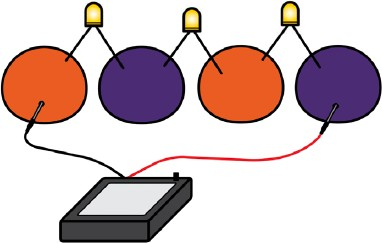
\includegraphics[width=4cm]{image 1.png}
\end{figure}
\item Label what kind of circuit the picture shows. \underline{Parallel}

\begin{figure}[h!]
\centering
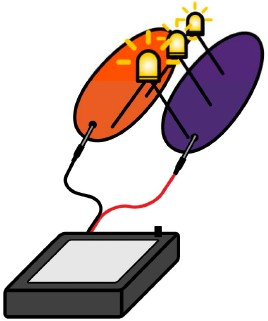
\includegraphics[width=4cm]{image 2.png}
\end{figure}
\end{enumerate}

\textit{Note:} Underlined words were fill-in-the-blank with answers being present in a word bank.
\end{large}
\end{document}
